\documentclass[xcolor=dvipsnames]{beamer}
% \usetheme{CambridgeUS}
% \useinnertheme{rectangles}
% \useoutertheme{infolines}
% \usecolortheme[named=Brown]{structure}
\definecolor{UniBlue}{RGB}{100,80,200}
\setbeamercolor{title}{fg=UniBlue}
\setbeamercolor{frametitle}{fg=UniBlue}
\setbeamercolor{structure}{fg=UniBlue}
\usepackage[utf8]{inputenc}
\usepackage{minted}
\usepackage{tikz}
\usepackage{graphicx}
\usepackage{caption}
\usepackage{subcaption}
\usepackage[tt=false]{libertine}
\def\checkmark{\tikz\fill[scale=0.4](0,.35) -- (.25,0) -- (1,.7) -- (.25,.15) -- cycle;} 
\def\CC{{C\nolinebreak[4]\hspace{-.05em}\raisebox{.4ex}{\tiny\bf ++}}}


\title{\textsc{Citadel}: A Trusted Reference Monitor for Linux using Intel SGX Enclaves}
\author{A.H.~Bell-Thomas}
\institute{Computer Laboratory, University of Cambridge}
\date{\scriptsize $26^{\text{th}}$ June, 2020}

\begin{document}

\frame{\titlepage}

\begin{frame}{Background}
\pause
{\large
\begin{enumerate}
    \item \textbf{Reference Monitor} \\
    \pause
    $\;\;\rightsquigarrow$ \textit{Information Flow Control}
    \pause
    \vspace{1cm}
    \item \textbf{Intel SGX}
\end{enumerate}
}
\end{frame}

\begin{frame}{Information Flow Control}
    \begin{itemize}
        \item Access Control specifics \textit{who} can access resources. IFC also mediates \textit{how} they can be used once opened.
        \vspace{5mm}
        \item Construct an abstract system of \textit{entities}; \\
        $\;\;\rightsquigarrow$ processes, files, sockets, etc.
        \vspace{5mm}
        \item Each \textit{entity} carries a \textit{security context}, defining its granular ownership or restriction information.
        \vspace{5mm}
        \item Aim: achieve \textit{non-interference} between all \textit{security contexts}.
    \end{itemize}  
\end{frame}

\begin{frame}{Information Flow Control}  
    \textit{Very briefly;}
    \vspace{3mm}
    \begin{itemize}
        \item \textbf{Tagging} \\
        Entities must be uniquely and reliably identifiable to support decisions.
        \vspace{5mm}
        \item \textbf{Tracking} \\
        Contexts are mutable to accommodate an evolving situation.
        \vspace{5mm}
        \item \textbf{Policy Decisions} \\
        Is an operation acceptable given its consequences? \\
        e.g. $A \rightarrow B \iff A_s \preceq B_s \;\land\; A_i \succeq B_i$ \\
        c.f. Biba, Bell-LaPadula
    \end{itemize}
\end{frame}

\begin{frame}{\textit{Decentralised} Information Flow Control}
    \begin{itemize}
        \item Centrally administered systems are highly restrictive.
        \vspace{5mm}
        \item Idea: let entities specify their own protection policy for assets they own. Enforcement becomes \textit{discretionary}, allowing more flexibility and support for operations such as \textit{declassification}.
    \end{itemize}
    \vspace{5mm}
    Enforcement is implemented using a \textit{reference monitor}.
\end{frame}

\begin{frame}{Linux Security Modules}

    \begin{figure}[]
        \centering
        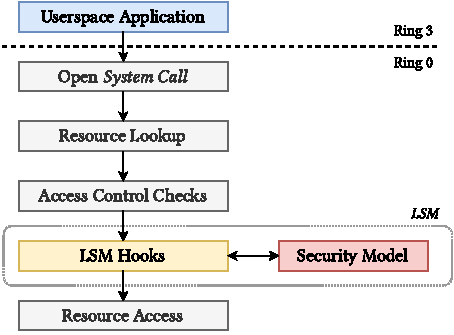
\includegraphics[width=0.6\linewidth]{../figures/LSM.pdf}
        \vspace{5mm}
        \caption{High level overview of the \textsc{Citadel} architecture.}
        \label{fig:citadel-overview}
    \end{figure}

\end{frame}

\begin{frame}{Intel SGX}
    A general-purpose \textit{trusted execution environment} provided via x86 at the architectural level in modern processors.
    \vspace{5mm}
    \begin{figure}[]
        \centering
        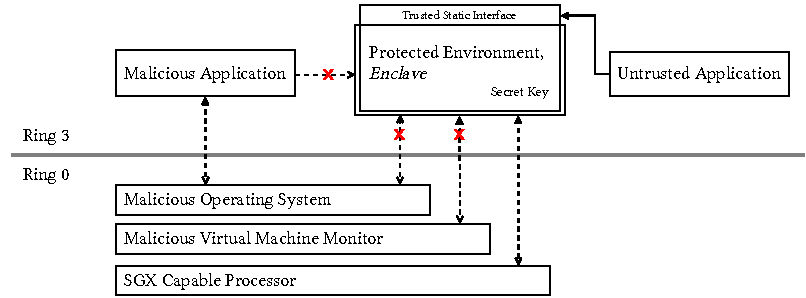
\includegraphics[width=0.99\linewidth]{../figures/SGX-architecture.pdf}
        \vspace{5mm}
        \caption{High level overview of the \textsc{Citadel} architecture.}
        \label{fig:citadel-overview}
    \end{figure}
\end{frame}


\begin{frame}{Intel SGX}
    \begin{figure}[]
        \centering
        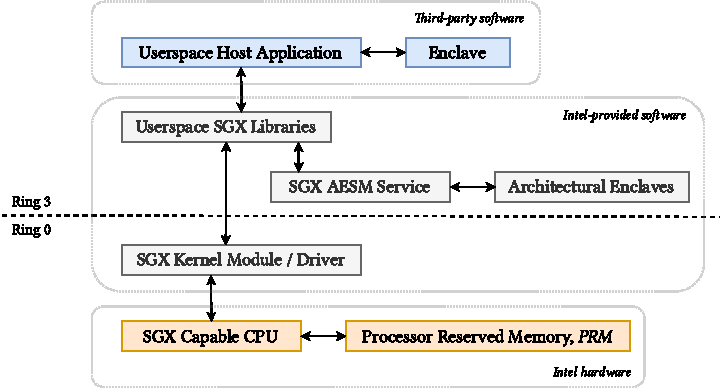
\includegraphics[width=0.99\linewidth]{../figures/SGX-AdvArchitecture.pdf}
        \vspace{5mm}
        \caption{High level overview of the \textsc{Citadel} architecture.}
        \label{fig:citadel-overview}
    \end{figure}
\end{frame}

\begin{frame}{\textsc{Citadel}}
    A prototype implementation of an SGX-protected reference monitor for Linux. \\ \\
    Reference monitors must be;
    \begin{itemize}
        \item Always invoked.
        \item Evaluable.
        \item Tamper proof.
    \end{itemize}
    \vspace{5mm}
    \textit{---  in theory, a perfect use case for SGX}.
\end{frame}

\begin{frame}{Architecture}

    \begin{figure}
        \centering
        \begin{subfigure}{.5\textwidth}
          \centering
          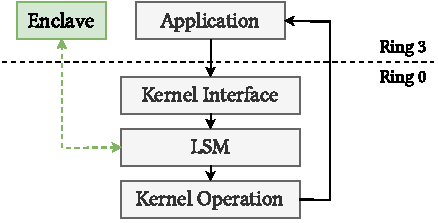
\includegraphics[width=.9\linewidth]{../figures/SGX-EnclaveIntegration.pdf}
          \vspace{5mm}
          \caption{A subfigure}
          \label{fig:sub1}
        \end{subfigure}%
        \begin{subfigure}{.5\textwidth}
          \centering
          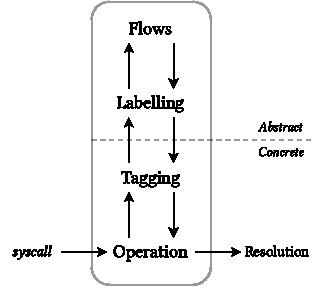
\includegraphics[width=.85\linewidth]{../figures/IFCFlow-1.pdf}
          \vspace{5mm}
          \caption{A subfigure}
          \label{fig:sub2}
        \end{subfigure}
        % \caption{A figure with two subfigures}
        \label{fig:test}
    \end{figure}

    
\end{frame}

\begin{frame}{Architecture}

    \begin{figure}
        \centering
        \begin{subfigure}{.5\textwidth}
          \centering
          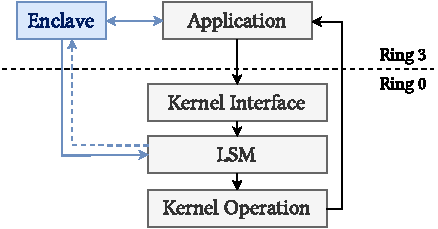
\includegraphics[width=.9\linewidth]{../figures/SGX-EnclaveIntegration-SoloActual.pdf}
          \vspace{5mm}
          \caption{A subfigure}
          \label{fig:sub1}
        \end{subfigure}%
        \begin{subfigure}{.5\textwidth}
          \centering
          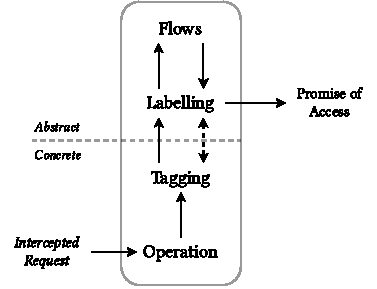
\includegraphics[width=\linewidth]{../figures/IFCFlow-2.pdf}
          \vspace{5mm}
          \caption{A subfigure}
          \label{fig:sub2}
        \end{subfigure}
        % \caption{A figure with two subfigures}
        \label{fig:test}
    \end{figure}

    
\end{frame}

\begin{frame}{Architecture}
\begin{figure}[]
    \centering
    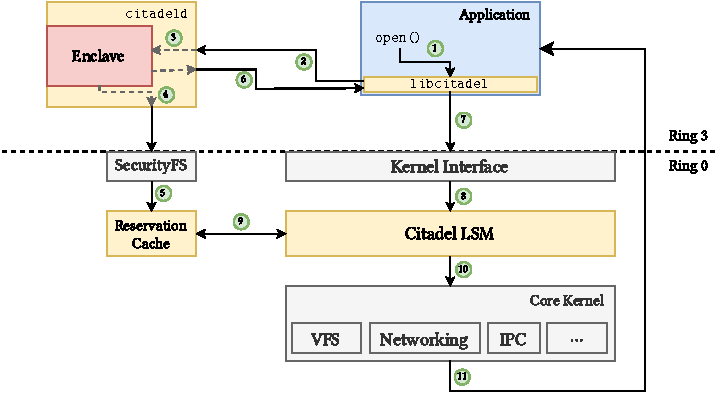
\includegraphics[width=\linewidth]{../figures/OverallArchitecture.pdf}
    % \vspace{5mm}
    % \caption{High level overview of the \textsc{Citadel} architecture.}
    \label{fig:citadel-overview}
\end{figure}
\end{frame}



\begin{frame}{Results}
    \begin{figure}[]
        \centering
        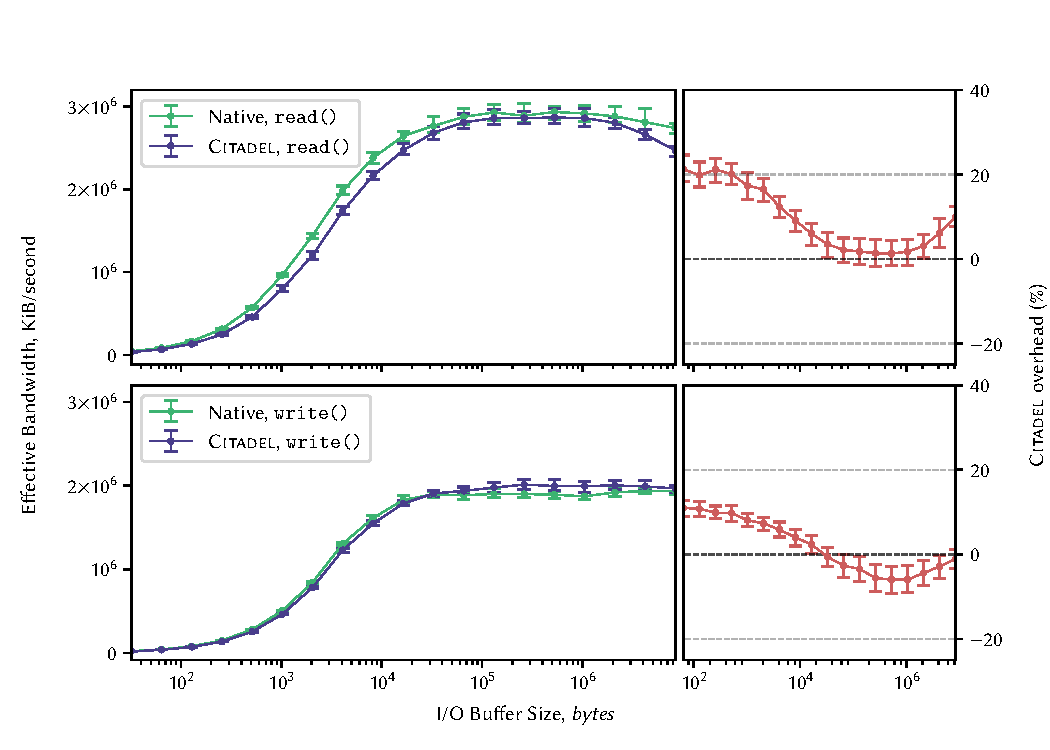
\includegraphics[width=0.9\linewidth]{../figures/graphs/io.pdf}
        \vspace{3mm}
        \caption{High level overview of the \textsc{Citadel} architecture.}
        \label{fig:citadel-overview}
    \end{figure}
\end{frame}

\begin{frame}{Results}
    \begin{itemize}
        \item Median \textit{syscall} overhead of $43\mu s\;\;$ ($1-2 \mu s$ amoritsed). \\ 
        \vspace{5mm}
        \item $20-25\%$ effective throughput decrease for IPC. \\ 
        \vspace{5mm}
        \item Real-world benchmarks using \textsc{Nginx};
        \begin{itemize}
            \item Low latency trials: 24\% median overhead.
            \item High bandwidth file transfers: $\sim 0\%$ median overhead.
        \end{itemize}

        
        \vspace{5mm}
        \item Security characteristics --- \textit{promising}.
    \end{itemize}
\end{frame}

\begin{frame}{Conclusion}
    \begin{itemize}
        \item \textsc{Citadel} ---  a modular, enclave-backed reference monitor to securely and verifiably implement IFC methods in the Linux kernel.
        \item Implemented using enclaves, an LSM, and an auxiliary library for unobstrusive application integration.
        \item Real-world performance overhead of $20-25\%$ observed using \textsc{Nginx} and microbenchmarks.
        \item Demonstrated the viability of a symbiotic enclave-kernel relationship.
    \end{itemize}
\end{frame}

\begin{frame}{References}
    
\end{frame}


\end{document}

